\documentclass[]{article}
\usepackage{lmodern}
\usepackage{amssymb,amsmath}
\usepackage{ifxetex,ifluatex}
\usepackage{fixltx2e} % provides \textsubscript
\ifnum 0\ifxetex 1\fi\ifluatex 1\fi=0 % if pdftex
  \usepackage[T1]{fontenc}
  \usepackage[utf8]{inputenc}
\else % if luatex or xelatex
  \ifxetex
    \usepackage{mathspec}
  \else
    \usepackage{fontspec}
  \fi
  \defaultfontfeatures{Ligatures=TeX,Scale=MatchLowercase}
\fi
% use upquote if available, for straight quotes in verbatim environments
\IfFileExists{upquote.sty}{\usepackage{upquote}}{}
% use microtype if available
\IfFileExists{microtype.sty}{%
\usepackage{microtype}
\UseMicrotypeSet[protrusion]{basicmath} % disable protrusion for tt fonts
}{}
\usepackage[margin=1in]{geometry}
\usepackage{hyperref}
\hypersetup{unicode=true,
            pdftitle={Introduction},
            pdfborder={0 0 0},
            breaklinks=true}
\urlstyle{same}  % don't use monospace font for urls
\usepackage{graphicx,grffile}
\makeatletter
\def\maxwidth{\ifdim\Gin@nat@width>\linewidth\linewidth\else\Gin@nat@width\fi}
\def\maxheight{\ifdim\Gin@nat@height>\textheight\textheight\else\Gin@nat@height\fi}
\makeatother
% Scale images if necessary, so that they will not overflow the page
% margins by default, and it is still possible to overwrite the defaults
% using explicit options in \includegraphics[width, height, ...]{}
\setkeys{Gin}{width=\maxwidth,height=\maxheight,keepaspectratio}
\IfFileExists{parskip.sty}{%
\usepackage{parskip}
}{% else
\setlength{\parindent}{0pt}
\setlength{\parskip}{6pt plus 2pt minus 1pt}
}
\setlength{\emergencystretch}{3em}  % prevent overfull lines
\providecommand{\tightlist}{%
  \setlength{\itemsep}{0pt}\setlength{\parskip}{0pt}}
\setcounter{secnumdepth}{0}
% Redefines (sub)paragraphs to behave more like sections
\ifx\paragraph\undefined\else
\let\oldparagraph\paragraph
\renewcommand{\paragraph}[1]{\oldparagraph{#1}\mbox{}}
\fi
\ifx\subparagraph\undefined\else
\let\oldsubparagraph\subparagraph
\renewcommand{\subparagraph}[1]{\oldsubparagraph{#1}\mbox{}}
\fi

%%% Use protect on footnotes to avoid problems with footnotes in titles
\let\rmarkdownfootnote\footnote%
\def\footnote{\protect\rmarkdownfootnote}

%%% Change title format to be more compact
\usepackage{titling}

% Create subtitle command for use in maketitle
\newcommand{\subtitle}[1]{
  \posttitle{
    \begin{center}\large#1\end{center}
    }
}

\setlength{\droptitle}{-2em}

  \title{Introduction}
    \pretitle{\vspace{\droptitle}\centering\huge}
  \posttitle{\par}
    \author{}
    \preauthor{}\postauthor{}
    \date{}
    \predate{}\postdate{}
  

\begin{document}
\maketitle

\hypertarget{introduction}{%
\section{Introduction}\label{introduction}}

\hypertarget{goal}{%
\subsection{Goal}\label{goal}}

The goal of this paper is to illustrate a combination of machine
learning, natural language processing and graph analysis techniques
applied to corporate email to identify potential witnesses in
litigation.

\hypertarget{background}{%
\section{Background}\label{background}}

\begin{quote}
In times of political turmoil, events can move from impossible to
inevitable without even passing through improbable.
\href{https://www.project-syndicate.org/commentary/canceling-brexit-becoming-inevitable-by-anatole-kaletsky-2018-12}{Anatole
Kalesky}
\end{quote}

\href{https://en.wikipedia.org/wiki/Enron}{Enron Corp.} and its
affiliates were engaged in energy-related businesses, as described in
its
\href{https://www.sec.gov/Archives/edgar/data/1024401/000102440101500010/ene10-k.txt}{Annual
Report on Form 10-K for the year ended December 31, 2000}

\begin{Verbatim}[frame=single]

*    the transportation of natural gas through pipelines to
markets throughout the United States;

*    the generation, transmission and distribution of
electricity to markets in the northwestern United States;

*    the marketing of natural gas, electricity and other
commodities and related risk management and finance services
worldwide;

*    the development, construction and operation of power
plants, pipelines and other energy related assets worldwide;

*    the delivery and management of energy commodities and
capabilities to end-use retail customers in the industrial
and commercial business sectors; and

*    the development of an intelligent network platform to
provide bandwidth management services and the delivery of
high bandwidth communication applications.

As of December 31, 2000, Enron employed approximately
20,600 persons.

    \end{Verbatim}

For the year ended December 31, 2000, it had operating revenues of
\$100,789 million, according to the same report.

On December 2, 2001, Enron filed for
\href{(https://www.sec.gov/Archives/edgar/data/1024401/000102440101500046/ene8-k1214.txt}{bankruptcy
protection}.

In less than a year, Enron underwent a complete reversal of fortune as
its business strategies ran afoul of applicable regulations, among which
were those of the Federal Energy Regulatory Commission (\textbf{FERC}).

FERC
\href{https://www.ferc.gov/industries/electric/indus-act/wec/chron/chronology.pdf}{became
aware} of irregularities in the California wholesale electricity market
prices. An orientation to the issues is provided by
\href{https://web.stanford.edu/group/fwolak/cgi-bin/sites/default/files/files/2002,\%20May\%2015_Senate\%20Committee\%20on\%20Commerce,\%20Science\%20and\%20Transportation_Wolak.pdf}{testimony}
before FERC, which provides a concise summary.\footnote{The short
  version, which I can relate as a former California regulatory official
  from personal knowledge, is that public electric utilities were losing
  a large share of industrial customers to self-generation. Many
  businesses found it cheaper to generate on-site than to pay tariff
  rates. Foreseeably, residential and business customers without the
  option to self-generate would come to bear the entire cost of
  unamortized utility fixed assets\footnote{Termed \emph{stranded costs}},
  and rates for retail, commercial and small industrial customers would
  increase. The adopted solution was to require the utilities to sell
  their generation plants and buy power on a new public market on a
  \emph{day-ahead}, tomorrow's estimated demand, and an
  \emph{hour-ahead} basis. Although much thought was devoted to the
  dangers that participants would game the system to sell or buy at
  discounts from market, insufficient consideration was given to
  mufti-participant cooperation.}

Following Enron's bankruptcy, FERC began an intense investigation,
including the email records of 149 Enron employees. A preliminary
\href{http://elibrary.ferc.gov/idmws/common/opennat.asp?fileID=9548231}{staff
report} issued six months later.

\hypertarget{motivating-data}{%
\subsection{Motivating Data}\label{motivating-data}}

FERC obtained approximately 500,000 emails. Copies of these were
acquired by Leslie Kaelbling of MIT and
\href{https://www.cs.cmu.edu/~./enron/}{published} by William W. Cohen
of Carnegie Mellon University. It is one of the largest publicly
available datasets of corporate email and is referred to as the Enron
Corpus. The term \emph{corpus} is used in natural language processing to
denote a collection of related text.

At the time, electronic record examination (\emph{ediscovery}) in
litigation was in a primitive state. It was not uncommon, for example,
for paper copies of email to be offered. These would typically be read
by teams of freelance attorneys looking for keywords. Advanced
technology included scanning with optical character recognition and some
proprietary software options to organize emails and capture the status
of review. Much of the focus was directed to keyword searches, sometimes
called the \emph{smoking gun} approach. Brute force examination misses
opportunities to understand the social networks that reflect how the
organization operates, what their concerns are and the haphazard
exposure of document reviewers inevitably poses the
\href{https://buddhismnow.com/2018/02/16/tittha-sutta-buddhist-parable-of-the-blind-men-and-the-elephant/}{Elephant
and the Blind Men Problem}. To triage the corpus quickly and
efficiently, it should first be be distilled and analyzed.

\hypertarget{analysis}{%
\section{Analysis}\label{analysis}}

\hypertarget{data-acquisition}{%
\subsection{Data acquisition}\label{data-acquisition}}

I obtained a copy of the \href{}{2009 version} of the corpus. It
contains copies of emails of a private nature that involve three users
have who since requested to be
\href{https://www.cs.cmu.edu/~./enron/DELETIONS.txt}{redacted}. I have
removed those 27 emails.\footnote{Most of my work on data wrangling and
  preliminary took place in 2018 in Python, relying heavily on the NLTK
  and networkx packages.}

\hypertarget{conversion}{%
\subsubsection{Conversion}\label{conversion}}

Each email was a plaintext file\footnote{Most had been generated by
  Microsoft Outlook, but some older emails were produced in IBM Notes,
  which created some character encoding issues.} Each user had a
directory tree similar to the one below.\footnote{This user had 10
  directories with 3048 files (the directory tree has been pruned to
  omit spurious detail) containing 12,147 lines and 69,226 words.}

\begin{figure}
\centering
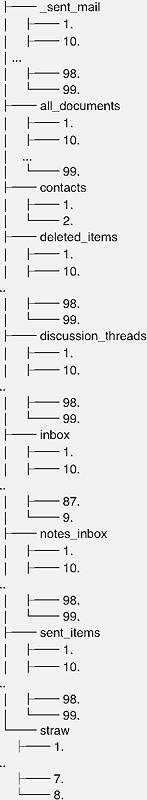
\includegraphics{https://s3-us-west-2.amazonaws.com/dslabs.nostromo/dtree.jpg}
\caption{Typical user data tree}
\end{figure}

Although tedious, traversing the directory tree, parsing the emails and
loading them into an SQL database, was accomplished with a combination
of Python and Perl scripting and standard bash tools. I do not reproduce
that process here as it has little bearing on the main topic of this
paper.

\hypertarget{data-structure}{%
\subsubsection{Data structure}\label{data-structure}}

While the emails were not in native format, the plain text versions
contained nine principal segments, as shown in the figure below

\begin{figure}
\centering
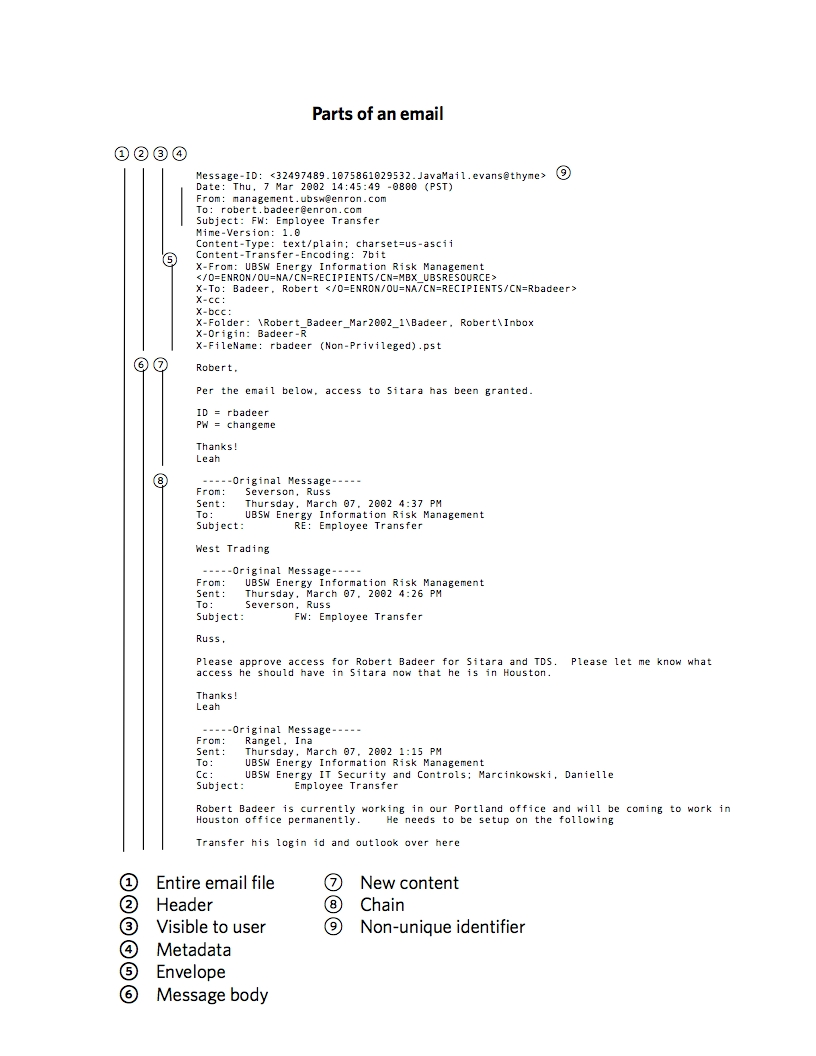
\includegraphics{https://s3-us-west-2.amazonaws.com/tuva/parse_email.png}
\caption{Structural analysis of an Enron email}
\end{figure}

Of those, the following were extracted from my earlier analysis for this
paper:

\begin{itemize}
\tightlist
\item
  sender
\item
  date
\item
  subject
\item
  recipient(s)
\item
  message body
\item
  new content
\end{itemize}

\hypertarget{deduplication}{%
\subsubsection{Deduplication}\label{deduplication}}

Using scripting tools, each text file extraction created a
\emph{payload} of the new content in the related email, capturing the
text between the beginning metadata and the following metadata for email
purposes. A \texttt{payload} hash, an
\href{https://en.wikipedia.org/wiki/MD5}{md5} encoded message
digest\footnote{In theory, it is possible that two non-identical
  sequences of bytes be encoded identically; the probability is low
  enough to make an md5 digest usable as a checksum verification, its
  purpose here.} was used in the initial analysis as a primary key to
assure the uniqueness of each record. Approximately half of the corpus
consisted of duplicates, such as the original message in the sender's
sent file and one or more copies in the recipient's inbox, at a minimum.
Multiple recipients and recipients who used email folders as a filing
system were another source of duplicate messages. Applying this filter
reduced the corpus to approximately 250,000 emails.

\hypertarget{text-isolation}{%
\subsubsection{Text isolation}\label{text-isolation}}

For natural language processing (\textbf{NLP}) purposes, treating the
\texttt{payload} rather than the \texttt{message\ body} as the unit of
analysis avoided an \emph{echo chamber} effect of \texttt{chains}
quoting and re-quoting the original message, multiplying the frequency
of the words it contained.

\hypertarget{prioritization}{%
\subsubsection{Prioritization}\label{prioritization}}

Traditional analysis of emails was conducted on the principe that
\emph{something may be overlooked,} which delays the value of email in
preliminary analysis. Prioritizing always leaves open the option of
reviewing the set-asides later.

After deduplication, the first filter applied was to eliminate all email
from external addresses that were not also recipients from internal
addresses. Spam, newsletters and the like have low information
potential. This filter reduced the remaining half of the corpus by half
again, leaving approximately 125,000 emails.

A second filter for internal email was used to eliminate broadcast
messages and high frequency administrative messages. Indicia of
broadcast messages were large numbers of recipients, high frequency,
paucity of return correspondence and keyword in context screening.
Administrative messages to single recipients were identified by
frequency, lack of return correspondence and high frequency words. Many
of these were nagging emails concerning the lack of approval of expense
reports, for example. This filter reduced the dataset to approximately
24,000.

The third filter limited the dataset to emails sent before Enron's
December 2, 2001 bankruptcy. This filter reduced the email count to
approximately 13,500, about 2.7\% of the original total.\footnote{\emph{Ninety
  percent of everything is crap.} Theodore Sturgeon's Revelation, made
  in a dominantly paper-based information environment. \emph{See also}
  Pareto distributions.} A few emails dated ``1979-12-31'' were reviewed
and deleted.\footnote{In the technology of the day, user desktop
  computers relied on an internal clock powered by a battery; when the
  battery died, the date reset to what the operating system, usually a
  variant of Windows, considered as the beginning of time.} The
resulting dataset was named \texttt{g\_enron} for its primary purpose,
network graph analysis

\hypertarget{augmentation-and-transformation}{%
\subsubsection{Augmentation and
transformation}\label{augmentation-and-transformation}}

Each unique Enron address in the reduced dataset was assigned a userid.
The primary purpose was to facilitate social network analysis with node
identifiers of uniform length; the second, to reduce analyst bias
arising from gender stereotyping, frequency of exposure and similar
subjective pattern seeking behaviors.

The next transformation was to create an additional field with a
\texttt{corpus} object to facilitate natural language processing.

\begin{verbatim}
g_enron <- g_enron %>% mutate(edge_corp = map(payload, tm::VectorSource)
\end{verbatim}

To achieve a computationally practicable dataset for initial social
network analysis, emails were limited to single Enron sender to Enron
single recipient, reducing the dataset further, to 9,615 emails. The
resulting graph had low density, and the the dataset was further trimmed
by restricting it to reciprocal correspondents, each of whom sent an
email to the other, either as a reply or an original message, excluding
emails by a user to herself. This further reduced the dataset, to 6,009
emails among 465 users. Finally, many emails were found to be blank or
extremely short -- fewer than 10 characters, resulting in a final count
of 5,922 emails among 445 users.

{[}latentnet{]}:Krivitsky PN, Handcock MS (2008). ``Fitting position
latent cluster models for social networks with latentnet.''
\emph{Journal of Statistical Software},
\url{https://CRAN.R-project.org/package=latentnet}


\end{document}
